
\section{Scatterplot Matrix: Time as a Grouping Variable \label{SEC:groupVariable}}
\label{sec:org8e8055b}

The scatterplot matrices are based on the technique of small multiples
\cite{Tufte1990}: small, thumbnail-sized representations of multiple
images displayed all at once, which allows the reader to immediately,
and in parallel, compare the inter-frame differences.  A scatterplot
matrix is a display of all pairwise bivariate scatterplots arranged in
a \(p \times p\) matrix for \(p\) variables. Each subplot shows the
relation between the pair of variables at the intersection of the row
and column indicated by the variable names in the diagonal panels
\cite{Friendly.Denis2005}.

This graphical tool is implemented in the \texttt{splom} function. The
following code displays the relation between the set of
meteorological variables using a sequential palette from the
ColorBrewer catalog (\texttt{RbBu}, with black added to complete a
twelve-color palette) to encode the month. The order of colors of
this palette is chosen in order to display summer months with
intense colors and to distinguish between the first and second
half of the year with red and blue, respectively (Figure
\ref{fig:aranjuezSplom}).

\index{splom@\texttt{splom}}


\lstset{language=r,label= ,caption= ,captionpos=b,numbers=none}
\begin{lstlisting}
library(zoo)

load('data/aranjuez.RData')
aranjuezDF <- as.data.frame(aranjuez)
aranjuezDF$Month <- format(index(aranjuez), '%m')
\end{lstlisting}

\lstset{language=r,label= ,caption= ,captionpos=b,numbers=none}
\begin{lstlisting}
## Red-Blue palette with black added (12 colors)
colors <- c(brewer.pal(n=11, 'RdBu'), '#000000')
## Rearrange according to months (darkest for summer)
colors <- colors[c(6:1, 12:7)]
\end{lstlisting}

\lstset{language=r,label= ,caption= ,captionpos=b,numbers=none}
\begin{lstlisting}
splom(~ aranjuezDF, 
      groups = aranjuezDF$Month,
      auto.key = list(space = 'right', 
                    title = 'Month', cex.title = 1),
      pscale = 0, varname.cex = 0.7, xlab = '',
      par.settings = custom.theme(symbol = colors,
                                pch = 19),
      cex = 0.3, alpha = 0.1)
\end{lstlisting}

\begin{figure}[htbp]
\centering
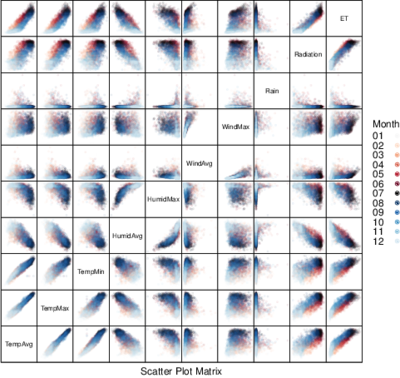
\includegraphics[width=.9\linewidth]{figs/aranjuezSplom.png}
\caption{Scatter plot matrix of the collection of meteorological time series of the Aranjuez station. \label{fig:aranjuezSplom}}
\end{figure}

A bit of interactivity can be added to this plot with the
identification of some points. This task is easy with
\texttt{panel.link.splom}. The points are selected via mouse clicks (and
highlighted in green). Clicks other than left-clicks terminate the
procedure. The output of this function is the index of chosen
points.

\index{panel.link.splom@\texttt{panel.link.splom}}
\index{trellis.focus@\texttt{trellis.focus}}

\lstset{language=r,label= ,caption= ,captionpos=b,numbers=none}
\begin{lstlisting}
trellis.focus('panel', 1, 1)
idx <- panel.link.splom(pch=13, cex=0.6, col='green')
aranjuez[idx,]
\end{lstlisting}

The \texttt{ggplot2} version of Figure \ref{fig:aranjuezSplom} is produced
thanks to the \texttt{ggpairs} function provided by the \texttt{GGally} package.

\index{ggpairs@\texttt{ggpairs}}
\index{Packages!GGally@\texttt{GGally}}

\lstset{language=r,label= ,caption= ,captionpos=b,numbers=none}
\begin{lstlisting}
library(GGally)

ggpairs(aranjuezDF,
        columns = 1:10, ## Do not include "Month"
        upper = list(continuous = "points"),
        mapping = aes(colour = Month, alpha = 0.1))
\end{lstlisting}

Let's explore Figure \ref{fig:aranjuezSplom}. For example,
\begin{itemize}
\item The highest values of ambient temperature (average, maximum, and
minimum), solar radiation, and evotranspiration can be found during
the summer.
\item These variables are almost linearly related. The relation between
radiation and temperature is different during both halves of the
year (red and blue regions can be easily distinguished).
\item The humidity reaches its highest values during winter without
appreciable differences between the first and second half of the
year. The temperature and humidity may be related with an
exponential function.
\end{itemize}

\subsection{Hexagonal Binning \label{SEC:hexbin}}
\label{sec:orgc9fccad}

For large datasets, the display of a large number of points in a
scatterplot produces hidden point density, long computation times,
and slow displays. These problems can be circumvented with the
estimation and representation of points densities.  A common
encoding uses gray scales, pseudo colors or partial
transparency. An improved scheme encodes density as the size of
hexagon symbols inscribed within hexagonal binning regions
\cite{Carr.Littlefield.ea1987}.

The \texttt{hexbin} package \cite{Carr.Lewin-Koh.ea2013} includes several
functions for hexagonal binning.  The \texttt{panel.hexbinplot} is a good
substitute for the default panel function. In addition, our first
attempt with \texttt{splom} can be improved with several modifications
(Figure \ref{fig:aranjuezSplomHexbin}):
\begin{itemize}
\item The scale's ticks and labels are suppressed with \texttt{pscale=0}.
\item The panels of the lower part of the matrix (\texttt{lower.panel}) will
include a locally weighted scatterplot smoothing (loess) with
\texttt{panel.loess}.
\item The diagonal panels (\texttt{diag.panel}) will display the kernel
density estimate of each variable. The \texttt{density} function
computes this estimate. The result is adjusted to the panel
limits (calculated with \texttt{current.panel.limits}). The kernel
density is plotted with \texttt{panel.lines} and the \texttt{diag.panel.splom}
function completes the content of each diagonal panel.
\item The point density is encoded with the palette \texttt{BTC} (ligther
colors for high density values and darker colors for almost
empty regions, with a gradient of blue hues for intermediate values).
\end{itemize}


\index{Packages!hexbin@\texttt{hexbin}}
\index{panel.hexbinplot@\texttt{panel.hexbinplot}}
\index{panel.loess@\texttt{panel.loess}}
\index{diag.panel.splom@\texttt{diag.panel.splom}}
\index{current.panel.limits@\texttt{current.panel.limits}}
\index{Panel function}


\lstset{language=r,label= ,caption= ,captionpos=b,numbers=none}
\begin{lstlisting}
library(hexbin)
  
splom(~as.data.frame(aranjuez),
      panel = panel.hexbinplot,
      colramp = BTC,
      diag.panel = function(x, ...){
          yrng <- current.panel.limits()$ylim
          d <- density(x, na.rm = TRUE)
          d$y <- with(d, yrng[1] + 0.95 * diff(yrng) * y / max(y))
          panel.lines(d)
          diag.panel.splom(x, ...)
      },
      lower.panel = function(x, y, ...){
          panel.hexbinplot(x, y, ...)
          panel.loess(x, y, ..., col = 'red')
      },
      xlab = '',
      pscale = 0, varname.cex = 0.7)
\end{lstlisting}

\begin{figure}[htbp]
\centering
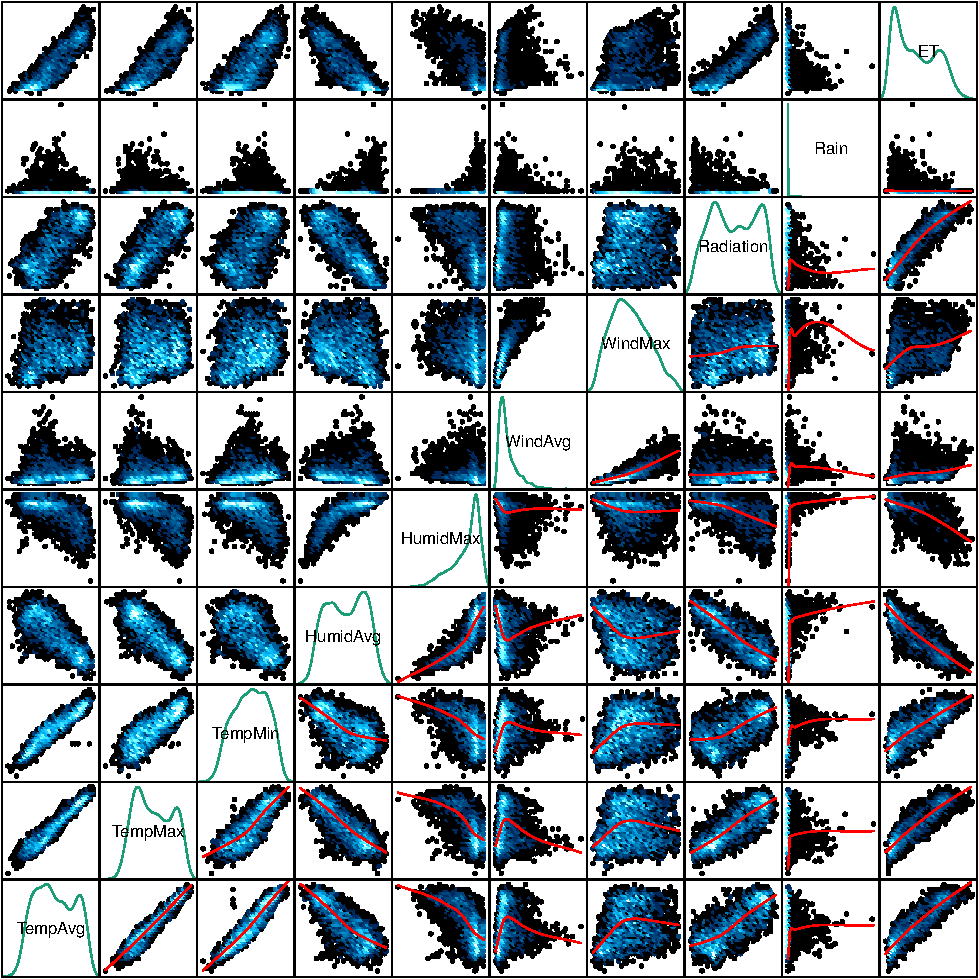
\includegraphics[width=.9\linewidth]{figs/aranjuezSplomHexbin.pdf}
\caption{Scatterplot matrix of the collection of meteorological time series of the Aranjuez station using hexagonal binning. \label{fig:aranjuezSplomHexbin}}
\end{figure}

A drawback of the matrix of scatterplots with hexagonal binning is
that each panel is drawn independently, so it is impossible to compute
a common color key for all of them. In other words, two cells with
exactly the same color in different panels encode different point
densities.

It is possible to display a reduced set of variables against another
one and generate a common color key using the \texttt{hexbinplot}
function. First, the dataset must be reshaped from the wide format
(one colum for each variable) to the long format (only one column for
the temperature values with one row for each observation). This task
is easily accomplished with the \texttt{melt} function included in the
\texttt{reshape2} package.

\index{melt\texttt{melt}}
\index{Packages!reshape2@\texttt{reshape2}}

\lstset{language=r,label= ,caption= ,captionpos=b,numbers=none}
\begin{lstlisting}
library(reshape2)

aranjuezRshp <- melt(aranjuezDF,
                     measure.vars = c('TempMax',
                                      'TempAvg',
                                      'TempMin'),
                     variable.name = 'Statistic',
                     value.name = 'Temperature')

summary(aranjuezRshp)
\end{lstlisting}

\begin{verbatim}
    HumidAvg        HumidMax         WindAvg         WindMax      
 Min.   :19.89   Min.   : 35.88   Min.   :0.250   Min.   : 1.550  
 1st Qu.:47.04   1st Qu.: 81.60   1st Qu.:0.670   1st Qu.: 3.780  
 Median :62.49   Median : 90.90   Median :0.920   Median : 5.030  
 Mean   :62.11   Mean   : 87.20   Mean   :1.166   Mean   : 5.216  
 3rd Qu.:77.30   3rd Qu.: 94.90   3rd Qu.:1.430   3rd Qu.: 6.540  
 Max.   :99.50   Max.   :100.00   Max.   :6.450   Max.   :10.000  
 NA's   :6       NA's   :33                       NA's   :345     
   Radiation          Rain              ET           Month          
 Min.   : 0.28   Min.   : 0.000   Min.   :0.000   Length:8694       
 1st Qu.: 9.37   1st Qu.: 0.000   1st Qu.:1.160   Class :character  
 Median :16.67   Median : 0.000   Median :2.750   Mode  :character  
 Mean   :16.73   Mean   : 1.046   Mean   :3.088                     
 3rd Qu.:24.63   3rd Qu.: 0.200   3rd Qu.:4.923                     
 Max.   :32.74   Max.   :49.730   Max.   :8.560                     
                                  NA's   :42                        
   Statistic     Temperature     
 TempMax:2898   Min.   :-12.980  
 TempAvg:2898   1st Qu.:  7.107  
 TempMin:2898   Median : 13.560  
                Mean   : 14.617  
                3rd Qu.: 21.670  
                Max.   : 41.910  
                NA's   :10
\end{verbatim}

The \texttt{hexbinplot} displays this dataset with a different panel for
each type of temperature (average, maximum, and minimum) but with a
common color key encoding the point density (Figure
\ref{fig:aranjuezHexbin}). Now, two cells with the same color in
different panels encode the same value. 

\index{hexbinplot@\texttt{hexbinplot}}
\index{Panel function}

\lstset{language=r,label= ,caption= ,captionpos=b,numbers=none}
\begin{lstlisting}
hexbinplot(Radiation ~ Temperature | Statistic,
           data = aranjuezRshp,
           layout = c(1, 3),
           colramp = BTC) +
    layer(panel.loess(..., col = 'red'))
\end{lstlisting}

\begin{figure}[htbp]
\centering
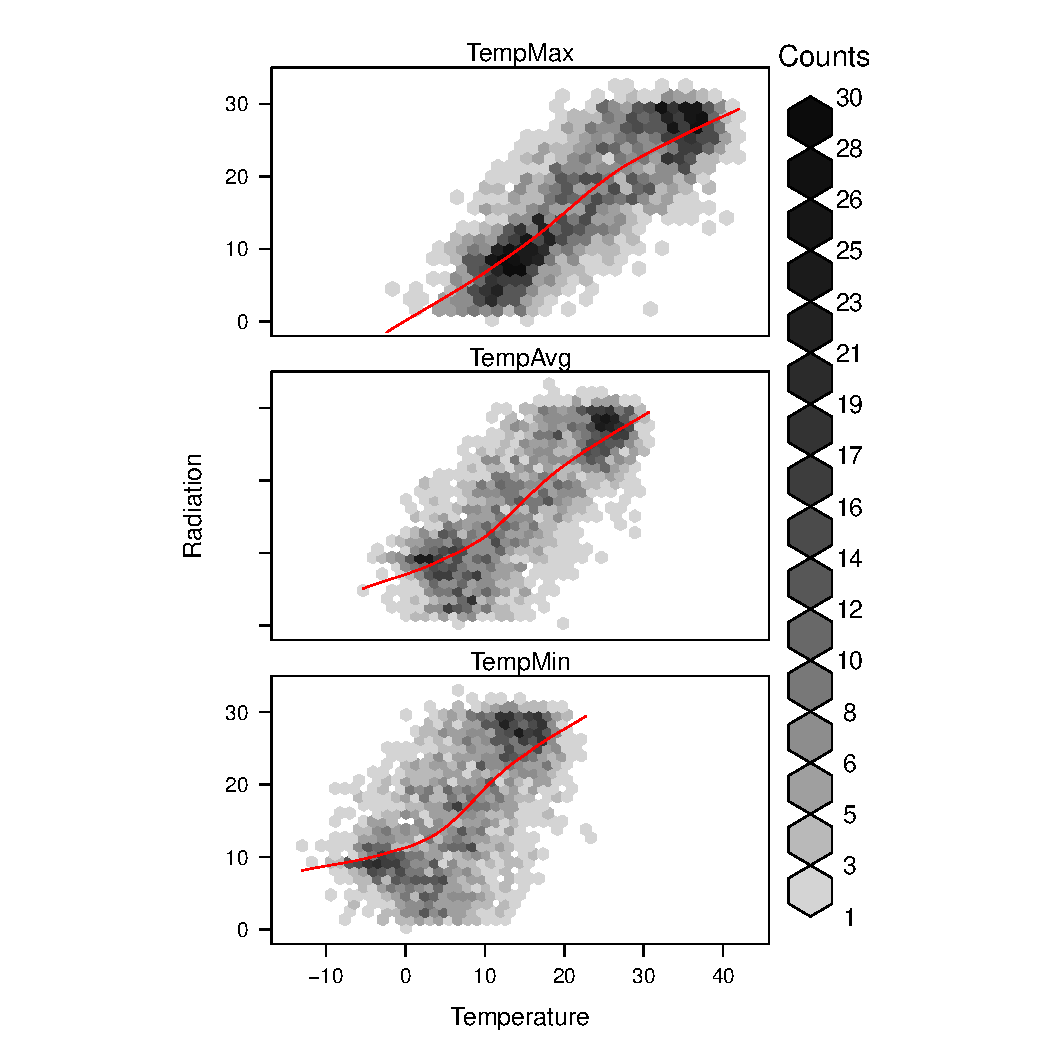
\includegraphics[width=.9\linewidth]{figs/aranjuezHexbinplot.pdf}
\caption{Scatterplot with hexagonal binning of temperature versus solar radiation using data of the Aranjuez station (\texttt{lattice} version). \label{fig:aranjuezHexbin}}
\end{figure}

The ggplot2 version is based on the \texttt{stat\_binhex} function.
\lstset{language=r,label= ,caption= ,captionpos=b,numbers=none}
\begin{lstlisting}
ggplot(data = aranjuezRshp,
       aes(Temperature, Radiation)) +
    stat_binhex(ncol = 1) + 
    stat_smooth(se = FALSE, method = 'loess', col = 'red') +
    facet_wrap(~ Statistic, ncol = 1) +
    theme_bw()
\end{lstlisting}

\section{Scatterplot with Time as a Conditioning Variable \label{SEC:conditionVariable}}
\label{sec:org0622301}

After discussing the hexagonal binning, let's recover the time
variable. Figure \ref{fig:aranjuezSplom} uses colors to encode
months. Instead, we will now display separate scatterplots with a
panel for each month. In addition, the statistic type (average,
maximum, minimum) is included as an additional conditioning variable.

This matrix of panels can be displayed with \texttt{ggplot} using
\texttt{facet\_grid}. The code of Figure \ref{fig:aranjuezFacetGrid} uses partial
transparency to cope with overplotting, small horizontal and vertical
segments (\texttt{geom\_rug}) to display points density on both variables, and
a smooth line in each panel.
\lstset{language=r,label= ,caption= ,captionpos=b,numbers=none}
\begin{lstlisting}
ggplot(data = aranjuezRshp, aes(Radiation, Temperature)) +
    facet_grid(Statistic ~ month) +
    geom_point(col = 'skyblue4', pch = 19, cex = 0.5, alpha = 0.3) +
    geom_rug() +
    stat_smooth(se = FALSE, method = 'loess', col = 'indianred1', lwd = 1.2) +
    theme_bw()
\end{lstlisting}

\begin{figure}[htbp]
\centering
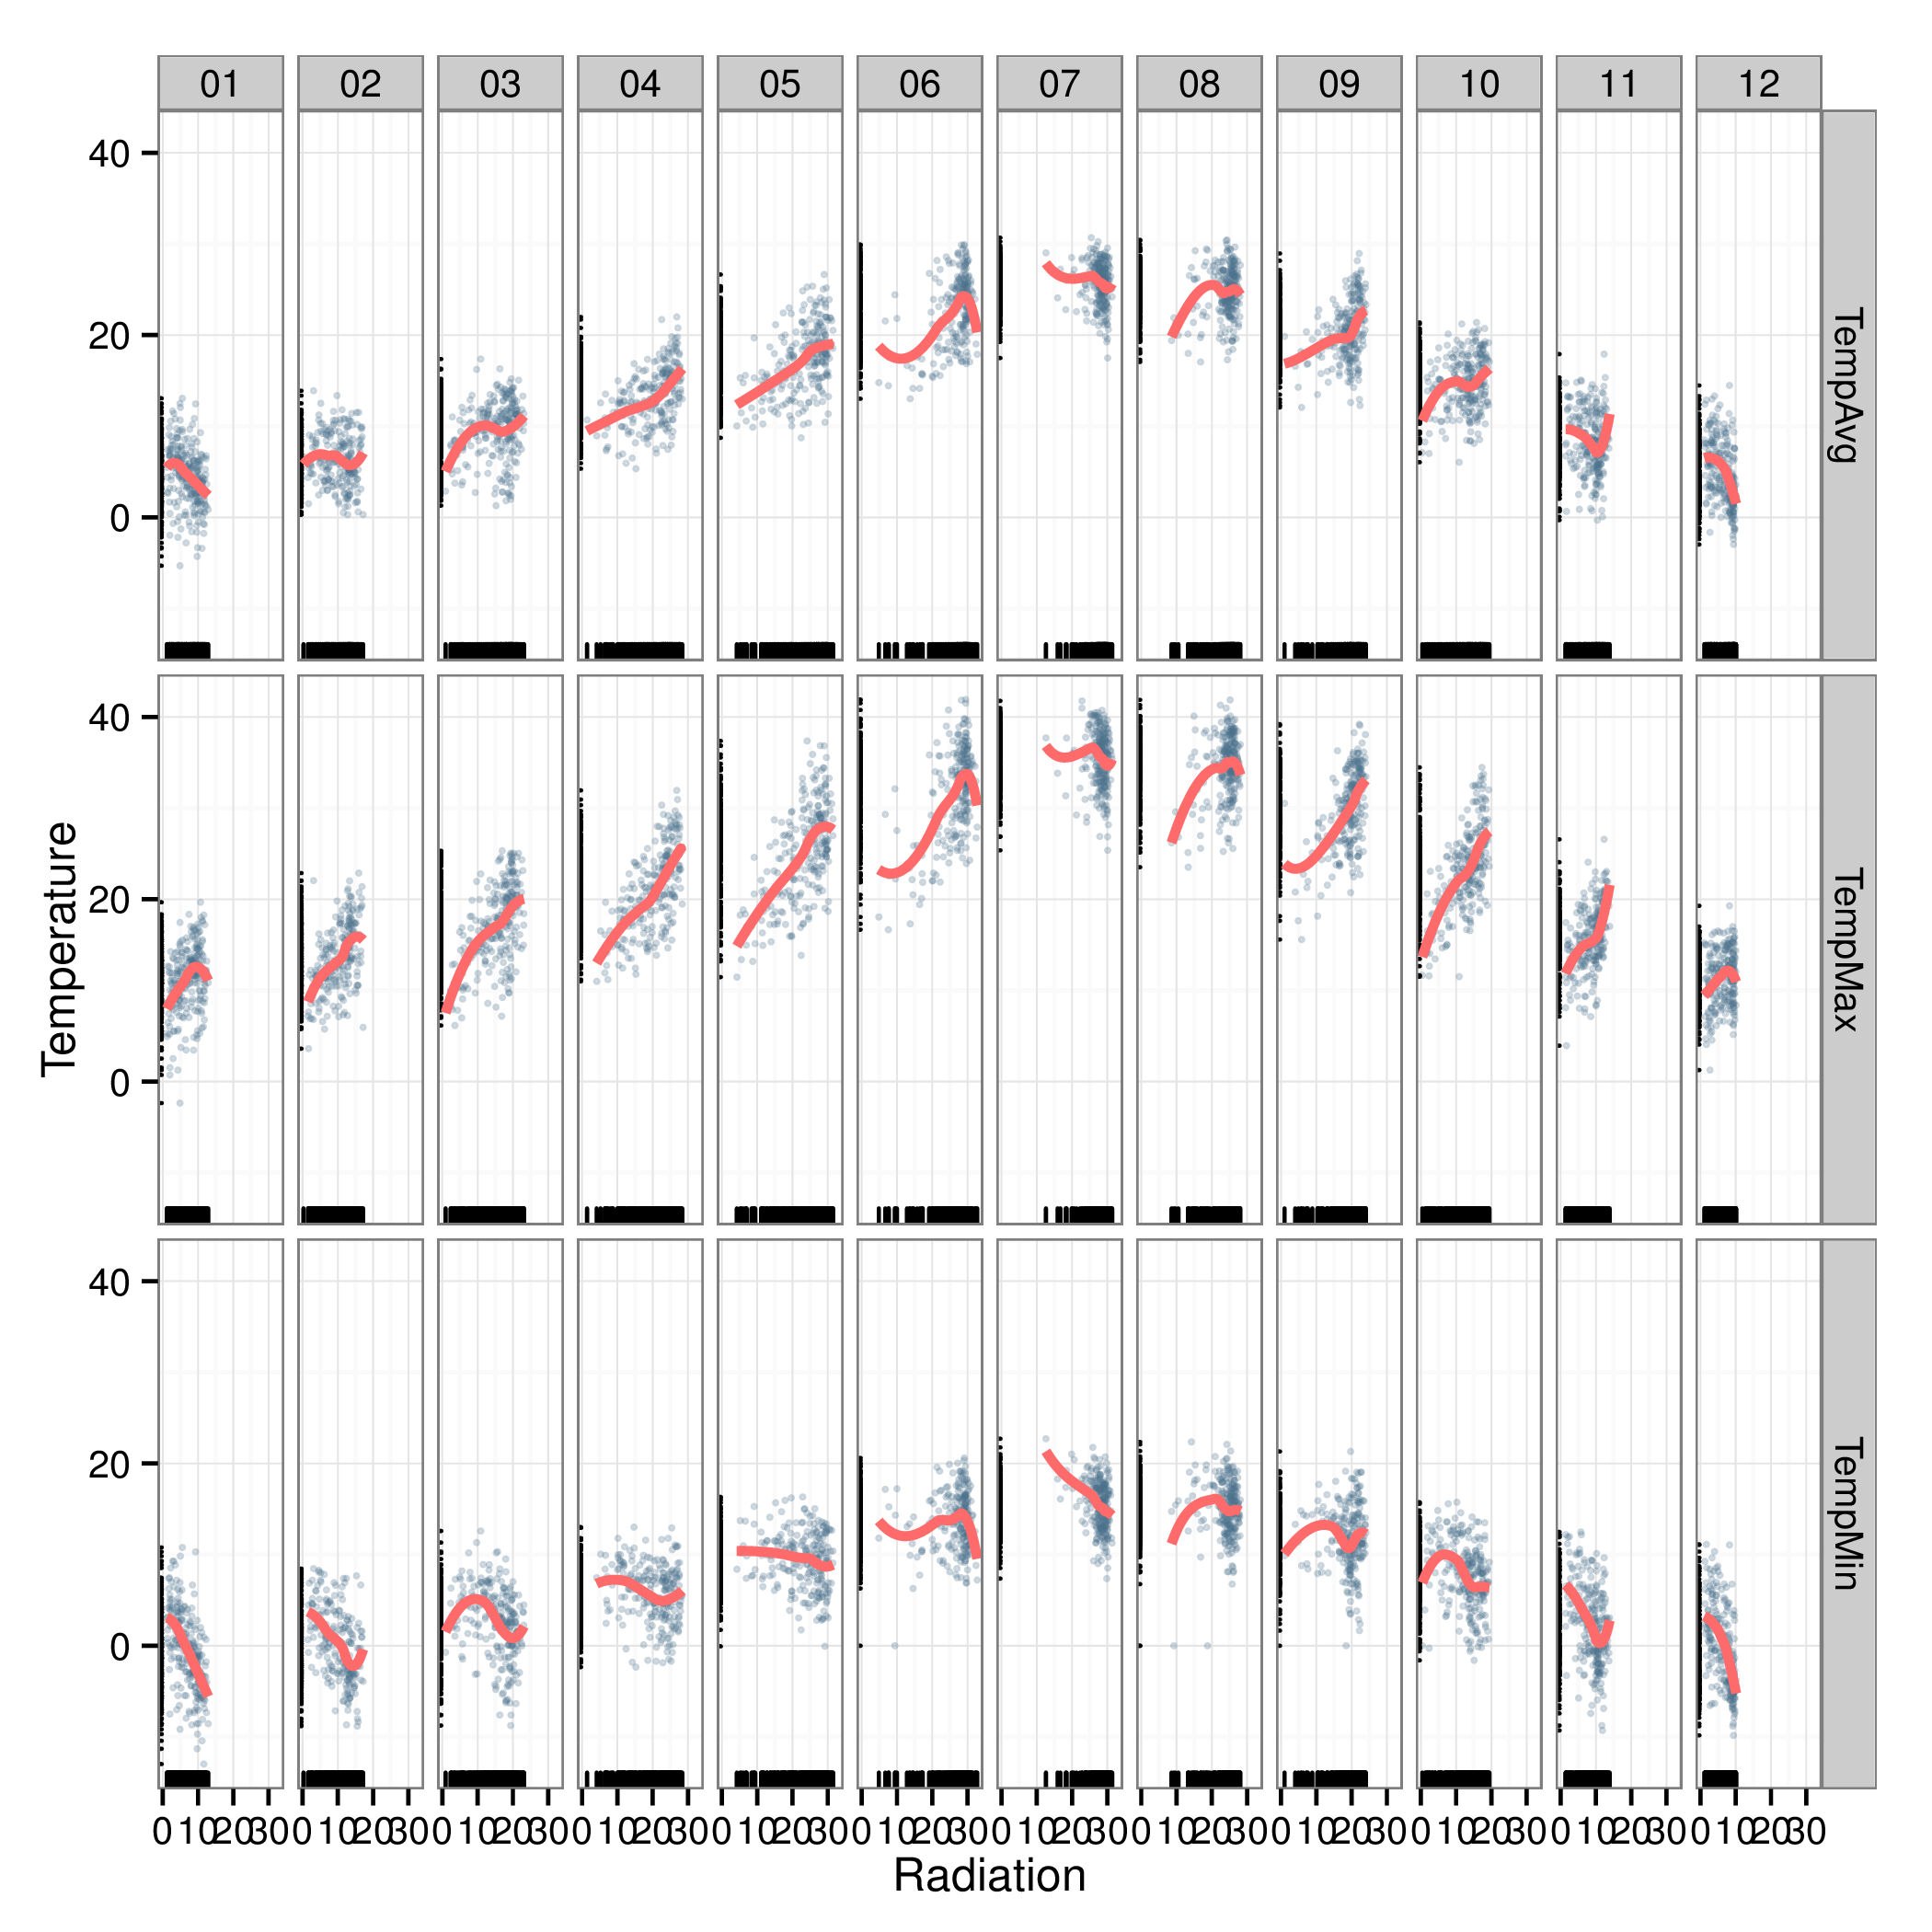
\includegraphics[width=.9\linewidth]{figs/aranjuezFacetGrid.png}
\caption{Scatterplot of temperature versus solar radiation for each month using data of the Aranjuez station (\texttt{ggplot2} version). \label{fig:aranjuezFacetGrid}}
\end{figure}

The version with \texttt{lattice} needs the \texttt{useOuterStrips} function from
the \texttt{latticeExtra} package, which prints the names of the conditioning
variables on the top and left outer margins (Figure
 \ref{fig:aranjuezOuterStrips}).

\index{useOuterStrips@\texttt{useOuterStrips}}
\index{panel.rug@\texttt{panel.rug}}
\index{panel.loess@\texttt{panel.loess}}
\index{Packages!latticeExtra@\texttt{latticeExtra}}

\lstset{language=r,label= ,caption= ,captionpos=b,numbers=none}
\begin{lstlisting}
useOuterStrips(xyplot(Temperature ~ Radiation | month * Statistic,
                      data = aranjuezRshp,
                      between = list(x = 0),
                      col = 'skyblue4', pch = 19,
                      cex = 0.5, alpha = 0.3)) +
    layer({
        panel.rug(..., col.line = 'indianred1', end = 0.05, alpha = 0.6)
        panel.loess(..., col = 'indianred1', lwd = 1.5, alpha = 1)
    })
\end{lstlisting}

\begin{figure}[htbp]
\centering
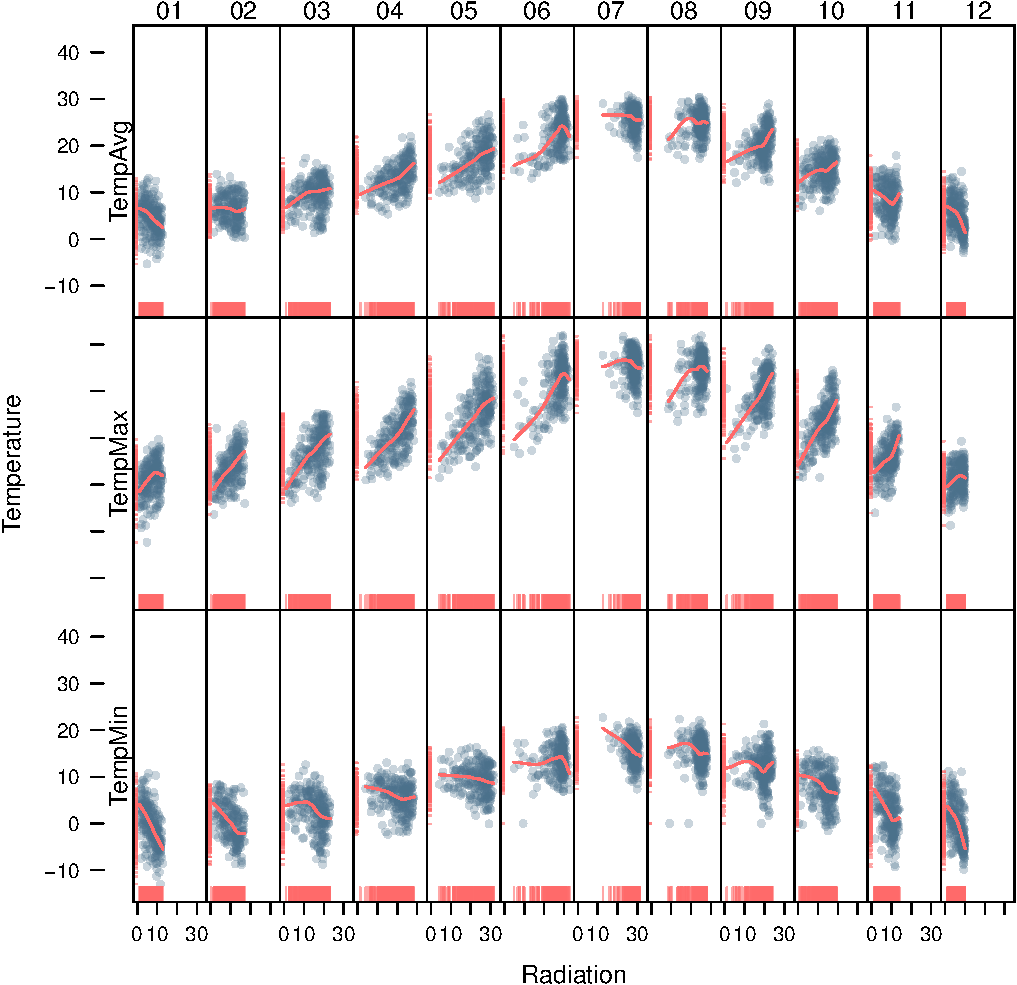
\includegraphics[width=.9\linewidth]{figs/aranjuezOuterStrips.pdf}
\caption{Scatterplot of temperature versus solar radiation for each month using data of the Aranjuez station (lattice version). \label{fig:aranjuezOuterStrips}}
\end{figure}

These figures show the typical seasonal behavior of solar radiation
and ambient temperature. Additionally, it displays in more detail the
same relations between radiation and temperature already discussed
with Figure \ref{fig:aranjuezHexbin}.
